% Created 2016-04-21 Thu 23:52
\documentclass[11pt]{article}
\usepackage[utf8]{inputenc}
\usepackage[T1]{fontenc}
\usepackage{fixltx2e}
\usepackage{graphicx}
\usepackage{longtable}
\usepackage{float}
\usepackage{wrapfig}
\usepackage{rotating}
\usepackage[normalem]{ulem}
\usepackage{amsmath}
\usepackage{textcomp}
\usepackage{marvosym}
\usepackage{wasysym}
\usepackage{amssymb}
\usepackage{hyperref}
\tolerance=1000
\date{\today}
\title{README}
\hypersetup{
  pdfkeywords={},
  pdfsubject={},
  pdfcreator={Emacs 24.5.1 (Org mode 8.2.10)}}
\begin{document}

\maketitle
\textbf{prep$_{\text{ruby}}$$_{\text{challenges}}$}

\href{http://www.vikingcodeschool.com/web-markup-and-coding/level-up-your-ruby-judo}{The Ruby challenge problems from the Markup and Coding course of the Viking Code School Prep Work}

\url{https://www.vikingcodeschool.com}

\section{Ruby Calisthenics}
\label{sec-1}

\subsection{Power}
\label{sec-1-1}

Write a method \emph{power} which takes two integers (\emph{base} and \emph{exponent}) and 
returns the \emph{base} raised to the power of \emph{exponent}. Do not use Ruby's "**"
operator for this!

\begin{verbatim}
> power(3,4)
=> 81 # (3*3*3*3)
\end{verbatim}

\begin{verbatim}
def power(base,exponent)
  # returns base raised to the power of exponent without the use of ** operator

  a = base
  b = exponent
  c = []

  b.times do
    c.push a
  end

  p c.inject(1) {|product, n| product * n}
end

power(3,4)
\end{verbatim}

\subsection{Factorial}
\label{sec-1-2}

Write a method \emph{factorial} which takes a number and returns the product of 
every number up to the current number multiplied together.

\begin{verbatim}
> factorial(5)
=> 120 # from 1*2*3*4*5
\end{verbatim}

\begin{verbatim}
def factorial(n)
  # Int => Int
  # Takes a number and returns the product of every number up to 
  # the current number multiplied together

  a = []

  n.downto(1).each do |i|
    a.push i
  end

  p a.inject(1) {|product, n| product * n}

end

factorial(5)
\end{verbatim}

\subsection{Uniques}
\label{sec-1-3}

Write a method \emph{uniques} which takes an array of items and returns the array
without any duplicates. Don't use Ruby's \emph{uniq} method.

\begin{verbatim}
uniques([1,5,"frog",2,1,3,"frog"])
=> [1,5,"frog",2,3]
\end{verbatim}

\begin{verbatim}
def uniques(array)
  # Array of Items => Array of Items
  # Takes an array, returns array with duplicate items removed.
  # Write without uniq

  no_dupes = []
  couples = array.combination(2)
  groups = array.group_by{|e| e}

  groups.each do |g|
    no_dupes.push(g[0])
  end

  p no_dupes
end

uniques([1,5,"frog",2,1,3,"frog"])
\end{verbatim}

\subsection{Combinations}
\label{sec-1-4}

Write a method \emph{combinations} which takes two arrays of strings and returns
an array with all of the combinations of the items in them, listing the first
items first.

\begin{verbatim}
> combinations(["on","in"],["to","rope"])
=> ["onto","onrope","into","inrope"]
\end{verbatim}

\begin{verbatim}
def combinations(ary1,ary2)
  # Ary(Str), Ary(Str) => Ary(Str)
  # Takes two arrays of strings, returns an array with all of the combinations
  # of the items in them, listing the first item first.

  a = ary1
  b = ary2

  c = []

  a.each do |s|
    b.each do |x|
      c.push "#{s}#{x}"
    end
  end

  p c
end

combinations(["on","in"],["to","rope"])
\end{verbatim}

\subsection{Primes}
\label{sec-1-5}

Write a method \emph{is$_{\text{prime}}$?} which takes in a number and returns \emph{true} if it 
is a prime number.

\begin{verbatim}
> is_prime?(7)
=> true
> is_prime?(14)
=> false
\end{verbatim}

\begin{verbatim}
def is_prime?(i)
  range = (i-1).downto(2)

  range.each do |a|
    #p i%a == 0
  end

  p range.any? {|a| i%a == 0}
end

is_prime?(7)
\end{verbatim}

\subsection{Rectangle Overlap}
\label{sec-1-6}

Write a method \emph{overlap} which takes two rectangles defined by the 
coordinates of their corners, e.g. \emph{[[0,0],[3,3]]} and \emph{[[1,1],[4,6]]},
and determines whether they overlap. You can assume all coordinates are 
positive integers.

\begin{verbatim}
> overlap( [ [0,0],[3,3] ], [ [1,1],[4,5] ] )
=> true
> overlap( [ [0,0],[1,4] ], [ [1,1],[3,2] ] )
=> false 
\end{verbatim}

It doesn't count as overlapping if their edges touch but they do not 
otherwise overwrite each other. As expressed by a sixth grade student:

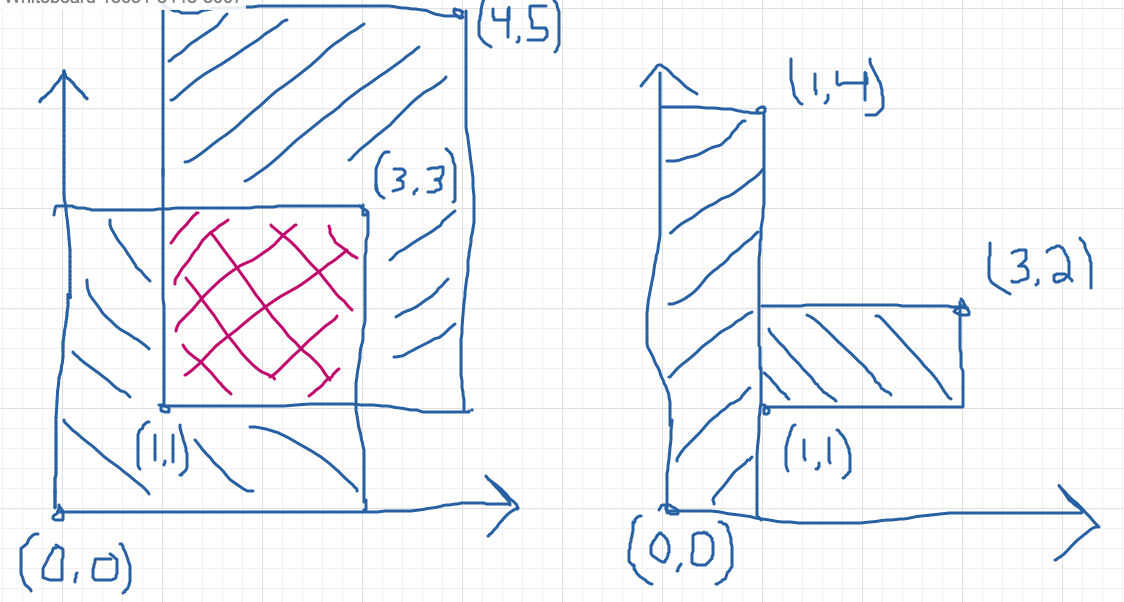
\includegraphics[width=.9\linewidth]{./coordinate_overlaps.png}

\begin{verbatim}
def overlap(a,b)
  # Array(Coordinates), Array(Coordinates) => Boolean

  # a = [[0,0],[3,3]]
  ax1 = a[0][0]
  ay1 = a[0][1] 
  ax2 = a[1][0]
  ay2 = a[1][1]

  awidth = ax2-ax1
  aheight = ay2-ay1
  aarea = awidth*aheight

  # b = [[1,1],[4,5]]
  bx1 = b[0][0]
  by1 = b[0][1]
  bx2 = b[1][0]
  by2 = b[1][1]

  bwidth = bx2-bx1
  bheight = by2-by1
  barea = bwidth*bheight

  #( [ [0  , 0  ],[3  , 3  ] ], [ [1  , 1  ],[4  , 5  ] ] )
  #( [ [ax1, ay1],[ax2, ay2] ], [ [bx1, by1],[bx2, by2] ] )

  case a
  when bx1 < ax2 && by1 < ay2
    true
  when bx1 < ax2 && by2 > ay1
    true
  when bx2 > ax1 && by2 > ay1
    true
  when ax1 < bx2 && ay2 > by1
    true
  else
    false
  end
end

p overlap( [ [0,0],[3,3] ], [ [1,1],[4,5] ] )
p overlap( [ [0,0],[1,4] ], [ [1,1],[3,2] ] )

# further development needed to explore every case
\end{verbatim}

\section{A Bigger Challenge: The Counting Game}
\label{sec-2}

10 friends are sitting in a circle around a table and decide to play a new 
game. In it, they count up through the numbers from 1 to 100. The first person
says "1", the second says "2" and so on\ldots{} but with a few catches:

\begin{itemize}
\item Whenever the number is divisible by 7, they switch directions. So person 6 
will say "6", person 7 will say "7", then person 6 again will say "8".

\begin{verbatim}
when x%y == 0 # reverse
\end{verbatim}

\item Whenever the number is divisible by 11, they skip the next person for the 
following number. For instance, if person 3 says "33", person 5 will say 
"34" instead (person 4 gets skipped).

\begin{verbatim}
friends = []
10.times do 
  friends.push 0
end
\end{verbatim}

\begin{verbatim}
# Produces each number and which person said it
# Hash {Person(Int)=>List of Numbers(Array of Integers)}
\end{verbatim}

\begin{verbatim}
friends = 10
persons = []

friends.times do
  persons.push []
end

count = 1

until count > 100
  persons.each_with_index do |person,index|
    id = index+1

    if count%7 > 0
      person.push count
    else
      person.push "#{count}, reverse"
    end

    p id
    p person
    count = count+1
  end

end
\end{verbatim}

\begin{verbatim}
nil
\end{verbatim}
\end{itemize}


Your job is to code a program which outputs each number and which person said 
it. Use it to show that  player 1 will say the number "100".

Tips:

\begin{itemize}
\item Remember to stick with brute force instead of trying to "figure out" the 
trick to the problem.
\item Name your variables well!
\item Ignore the skipping to start out with. Only add it when you're ready.
\end{itemize}


Advanced Option:

\begin{itemize}
\item Make your method take two inputs -- the number of players and the number 
you're counting up to. Then see who says the last number each time!
\end{itemize}




\subsection{The Elevator}
\label{sec-2-1}

You live in a 25 story building with one elevator. The central 
microcontroller got eaten by rats and the building manager has asked you to 
code up the elevator's operating procedure until he can get a new one. You 
figure you'll have to learn to actually code soon but you first want to think
things through and pseudocode your design.

\subsubsection{Elevator Details}
\label{sec-2-1-1}

The basic elevator machinery is completely dumb (it doesn't do anything it's
not told to do) but is capable of interpreting and executing the commands:

\begin{itemize}
\item "open elevator door"
\item "close elevator door"
\item "go up full speed"
\item "go down full speed"
\item "slow down"
\item "stop"
\end{itemize}


\ldots{}and it accepts user input in the form of:

\begin{itemize}
\item floor buttons inside the elevator
\item door open and close buttons inside the elevator
\item up and down call buttons on each floor
\end{itemize}


\ldots{}and it has sensors for:

\begin{itemize}
\item if a human is in the door closing path
\item if it is currently at a floor (instead of in-between floors)
\end{itemize}


\ldots{}and it has a few quirky requirements:

\begin{itemize}
\item it must "slow down" at least 1 floor before it stops.
\item there is a small chance that it actually stops between floors by 
accident (it's an old elevator)
\end{itemize}

\subsubsection{The Task}
\label{sec-2-1-2}

Your job is to design a properly working elevator. It should stop on each 
floor it is physically able to during a given trip to pick up whoever is 
going the same direction. Additionally, make sure that no one is:

\begin{enumerate}
\item smashed into the ground
\item pushed through the roof
\item squished by the doors
\item let off in between floors
\item stuck going the wrong direction (unless they choose not to exit)
\end{enumerate}


This will be good practice thinking about all the edge cases and scenarios 
that a user can do.

The point isn't to follow any strict guidelines of syntax but rather to 
focus on getting the logic of the problem figured out and then organizing it
into modules that accomplish the sub-tasks that are required.

Think about:

\begin{itemize}
\item Using a loop around everything to keep your pseudocode (and elevator) 
running.
\item Writing everything in one giant mess to start with and then refactoring it
to break apart the modules so it feels less cluttered and messy.
\end{itemize}

\subsubsection{Use Modules!}
\label{sec-2-1-3}

This exercise is large enough that you will need to break your code up into
modules. Remember the SOLID lessons -- modules should only have one major 
purpose. For this exercise, you can use other modules by simply calling 
their name in plain english and writing them out as separate programs down
below your main program. They could be groups of procedural instructions 
like "slow down the elevator if necessary", which runs the 
"ReachedADestinationFloor?" program.

\url{https://en.wikipedia.org/wiki/SOLID}$_{\text{(object-oriented}_{\text{design}}\text{)}}$
\url{https://www.vikingcodeschool.com/software-engineering-basics/solid-design-principles}

\begin{verbatim}
PROGRAM Elevator:
    # other code
    slow down the elevator if necessary
    # other code
END

# other code

PROGRAM SlowDownIfNecessary
    IF we are traveling up at full speed
        IF we are only 1 floor away from the lowest destination floor
            slow down
        END
    ELSE IF we are traveling down at full speed
        IF we are only 1 floor away from the highest destination floor
            slow down
        END
    END
END
\end{verbatim}

\subsection{NB: Software Engineering}
\label{sec-2-2}

\url{https://www.vikingcodeschool.com/software-engineering-basics}

\begin{itemize}
\item "logic" way through problems
\begin{itemize}
\item pseudocoding ("whiteboarding")
\begin{itemize}
\item software design
\begin{itemize}
\item solve problem first THEN code the solution
\item break Problem apart into individual sub-processes called "Modules"
\begin{itemize}
\item Modules Interface
\begin{itemize}
\item keep modules as independent as practically possible (aim for low "Coupling")
\item make sure modules are all working towards the same goal (are highly "Cohesive")
\item try to keep modules insulated from how other modules actually do 
their job (keep them highly "Encapsulated")
\end{itemize}
\end{itemize}
\item SOLID principles
\end{itemize}
\end{itemize}

\item modular design and engineering best practices
\item 4-step engineering problem solving approach
\begin{enumerate}
\item Understand the problem
\item Plan a solution
\item Carry out that plan
\item Examine your results for accuracy
\end{enumerate}
\item Agile development
\begin{itemize}
\item project management technique / development philosophy
\item teams commonly work in short (1-2 week) sprints
\item XP and SCRUM, Agile techniques
\begin{itemize}
\item short cycle times
\item frequent client/user interaction
\begin{itemize}
\item keeps project focused on relevant tasks
\end{itemize}
\item XP
\begin{itemize}
\item pair programming
\begin{itemize}
\item pairing developers together at workstations
\end{itemize}
\end{itemize}
\end{itemize}
\item keep software user-driven
\item TDD
\end{itemize}
\end{itemize}
\end{itemize}

\subsubsection{Learning Modularity}
\label{sec-2-2-1}

\begin{itemize}
\item The 3 Characteristics of Good Modules

Essentially, there are just three important guidelines for how modules 
should operate and interact. These high level principles essentially guide
the theory behind modularity -- it's good to break things into pieces, 
those pieces shouldn't rely on each other for much, each piece should do 
its own thing, and pieces should talk to each other using pre-determined
interfaces.

Modules should have:

\begin{enumerate}
\item Low Coupling -- they should be minimally dependent on each other and 
communicate using specified interfaces

\item High Cohesion -- they should be focused completely on achieving the 
overall goal

\item High Encapsulation -- they shouldn't reveal their implementation 
details to anyone else (and shouldn't need to)
\end{enumerate}

\item 5 key engineering principles. SOLID

\begin{enumerate}
\item \textbf{Single Responsibility Principle (SRP)} 

modules should only exist to serve one purpose and may only change if 
that purpose is modified

\item \textbf{Open/Closed Principle (OCP)}

modules should be open for extension but closed to modification

\item \textbf{Liskov Substitution Principle (DIP)}

modules that inherit from a parent should not alter any of that 
parent's functionality

\item \textbf{Interface Segregation Principle (ISP)}

each different user of a module should get to access it via a 
specialized interface that only requires them to supply the minimal 
amount of information

\item \textbf{Dependency Inversion Principle (DIP)}

higher level modules should dictate the implementation details of lower
level modules, not the other way around
\end{enumerate}
\end{itemize}
% Emacs 24.5.1 (Org mode 8.2.10)
\end{document}
